%!TEX program = xelatex
%!TEX options=--shell-escape
\documentclass[12pt]{article}

%
\usepackage[scheme=plain]{ctex}
%
\usepackage{fontspec}
%
\usepackage[margin = 1in]{geometry}

%
\usepackage[dvipsnames]{xcolor}
\usepackage[many]{tcolorbox}

%
\usepackage{amsmath}
\usepackage{amssymb}
\usepackage{amsthm}
%
\usepackage{tensor}
%
\usepackage{slashed}
\usepackage{physics}
\usepackage{simpler-wick}

%
\usepackage[version=4]{mhchem}

%
\usepackage{mathtools}

%
\usepackage{bm}
\newcommand{\dbar}{\dif\hspace*{-0.18em}\bar{}\hspace*{0.2em}}
\DeclareMathAlphabet\mathbfcal{OMS}{cmsy}{b}{n}
%\usepackage{bbold}
\newcommand*{\dif}{\mathop{}\!\mathrm{d}}
\newcommand*{\euler}{\mathrm{e}}
\newcommand*{\imagi}{\mathrm{i}}

\renewcommand{\vec}[1]{\boldsymbol{\mathbf{#1}}}

\usepackage{caption}

\usepackage{enumitem}

%
\usepackage{mathrsfs}
\usepackage{dsfont}

%
\usepackage{hyperref}
\hypersetup{
    colorlinks=true,
    linkcolor=violet,
    filecolor=blue,      
    urlcolor=blue,
    citecolor=cyan,
}

%
\usepackage{graphicx}
%
\graphicspath{{image/}}


%
\usepackage{indentfirst}
%
\setlength{\parindent}{2em}
\linespread{1.25}

% 
% \setmainfont{Times New Roman}

\title{Note}
\author{Feng-Yang Hsieh}
\date{}

\begin{document}
\maketitle
\section{Generate di-Higgs samples in SM}% (fold)
\label{sec:generate_di_higgs_samples_in_sm}
	Generate the double Higgs events in the standard model by MadGraph with \verb+loop_sm+ model. Following are the MadGraph scripts for generating di-Higgs samples:
	\begin{verbatim}
	import model loop_sm
	generate p p > h h [QCD] QED^2<=99 QCD^2<=99
	output /home/r10222035/CPVDM/Di-Higgs-SM/di-Higgs-sm

	launch /home/r10222035/CPVDM/Di-Higgs-SM/di-Higgs-sm

	shower=OFF
	detector=OFF
	analysis=OFF
	done

	set run_card nevents 10000
	set run_card ebeam1 6500.0
	set run_card ebeam2 6500.0

	done
	\end{verbatim}

	\subsection{Variation with \texorpdfstring{$\kappa_\lambda$}{kappa_lambda}}% (fold)
	\label{sub:variation_with_kappa_lambda}
		Reference: \href{https://answers.launchpad.net/mg5amcnlo/+question/678406}{How to change the trilinear Higgs coupling in Madgraph?}

		The definition of $\kappa_\lambda$
		\begin{equation}
			\kappa_\lambda \equiv \frac{\lambda_{HHH}}{\lambda_{HHH}^{\text{SM}}}
		\end{equation}

		Following the below steps, we can add a parameter $\kappa_\lambda$ in the model
		\begin{enumerate}
			\item Go to the MadGraph model file directory. Copy \verb+loop_sm+ to \verb+my_loop_sm+.
			\item Go to \verb+my_loop_sm+ directory. 
			\item In \verb+parameters.py+, add a new parameter for $\kappa_\lambda$ by
				\begin{verbatim}
				khhh = Parameter(name = 'khhh',
					  nature = 'external',
					  type = 'real',
					  value = 1,
					  texname = '\\text{khhh}',
					  lhablock = 'SMINPUTS',
					  lhacode = [ 10 ])
				\end{verbatim}
			\item In \verb+vertices.py+, we can find the coupling for three Higgs vertex in the form \verb+GC_XX+. 
			\item In \verb+couplings.py+, multiply the value for \verb+GC_XX+ found in step 4 by \verb+khhh+.
			\item In \verb+restrict_default.dat+, add
				\begin{verbatim}
				10 2.000000e+00 # khhh 
				\end{verbatim}
				in Block SMINPUTS.
		\end{enumerate}

		Finish the above setting we can use the following scripts to generate di-Higgs samples:
			\begin{verbatim}
			import model my_loop_sm
			generate p p > h h [QCD] QED^2<=99 QCD^2<=99
			output /home/r10222035/CPVDM/Di-Higgs-SM/di-Higgs-sm-kappa

			launch /home/r10222035/CPVDM/Di-Higgs-SM/di-Higgs-sm-kappa

			shower=OFF
			detector=OFF
			analysis=OFF
			done

			set param_card khhh 1

			set run_card nevents 10000
			set run_card ebeam1 6500.0
			set run_card ebeam2 6500.0

			done
			\end{verbatim}

	% subsection variation_with_kappa_lambda (end)
	\subsection{Results}% (fold)
	\label{sub:di_Higgs_sample_generating_results}
		The cross sections of various $\kappa_\lambda$ are showed in Table \ref{tab:di-Higgs-SM-kappa-cross-section}.
		\begin{table}[htpb]
			\centering
			\caption{The cross sections of various $\kappa_\lambda$. My data is the results from MadGraph. The reference data is from \href{https://link.springer.com/content/pdf/10.1007/JHEP06(2019)066.pdf}{here}. }
			\label{tab:di-Higgs-SM-kappa-cross-section}
			\begin{tabular}{c|cc|c|cc|cc}
							 & \multicolumn{3}{c|}{13 TeV}                     & \multicolumn{4}{c}{14 TeV}                                     \\
							 & \multicolumn{2}{c|}{Cross section (fb)} &        & \multicolumn{2}{c|}{Cross section (fb)} &       &               \\
			$\kappa_\lambda$ & Ref.              & My data            & Ref./My& Ref.              & My data            &Ref./My& Ref. K-factor \\ \hline
			-1               & 116.71            & 74.62              & 1.564  & 136.91            & 87.93              & 1.56  & 1.86          \\
			0                & 62.51             & 41.96              & 1.490  & 73.64             & 49.45              & 1.49  & 1.79          \\
			1                & 27.84             & 20.27              & 1.373  & 32.88             & 24.05              & 1.37  & 1.66          \\
			2                & 12.42             & 9.56               & 1.299  & 14.75             & 11.34              & 1.30  & 1.56          \\
			2.4              & 11.65             & 8.33               & 1.399  & 13.79             & 9.90               & 1.39  & 1.65          \\
			3                & 16.28             & 9.81               & 1.660  & 19.07             & 11.55              & 1.65  & 1.90          \\
			5                & 81.74             & 43.55              & 1.877  & 95.22             & 50.68              & 1.88  & 2.14         
			\end{tabular}
		\end{table}

		The $m_{HH}$ distribution with various $\kappa_\lambda$ is presented in Figure \ref{fig:di-Higgs-SM-kappa-mhh}. In the left plot, the data is the parton level data from MadGraph. The right plot comes from the ATLAS reference. Here, the $\sqrt{s} = \text{13 TeV}$
		\begin{figure}[htpb]
			\centering
			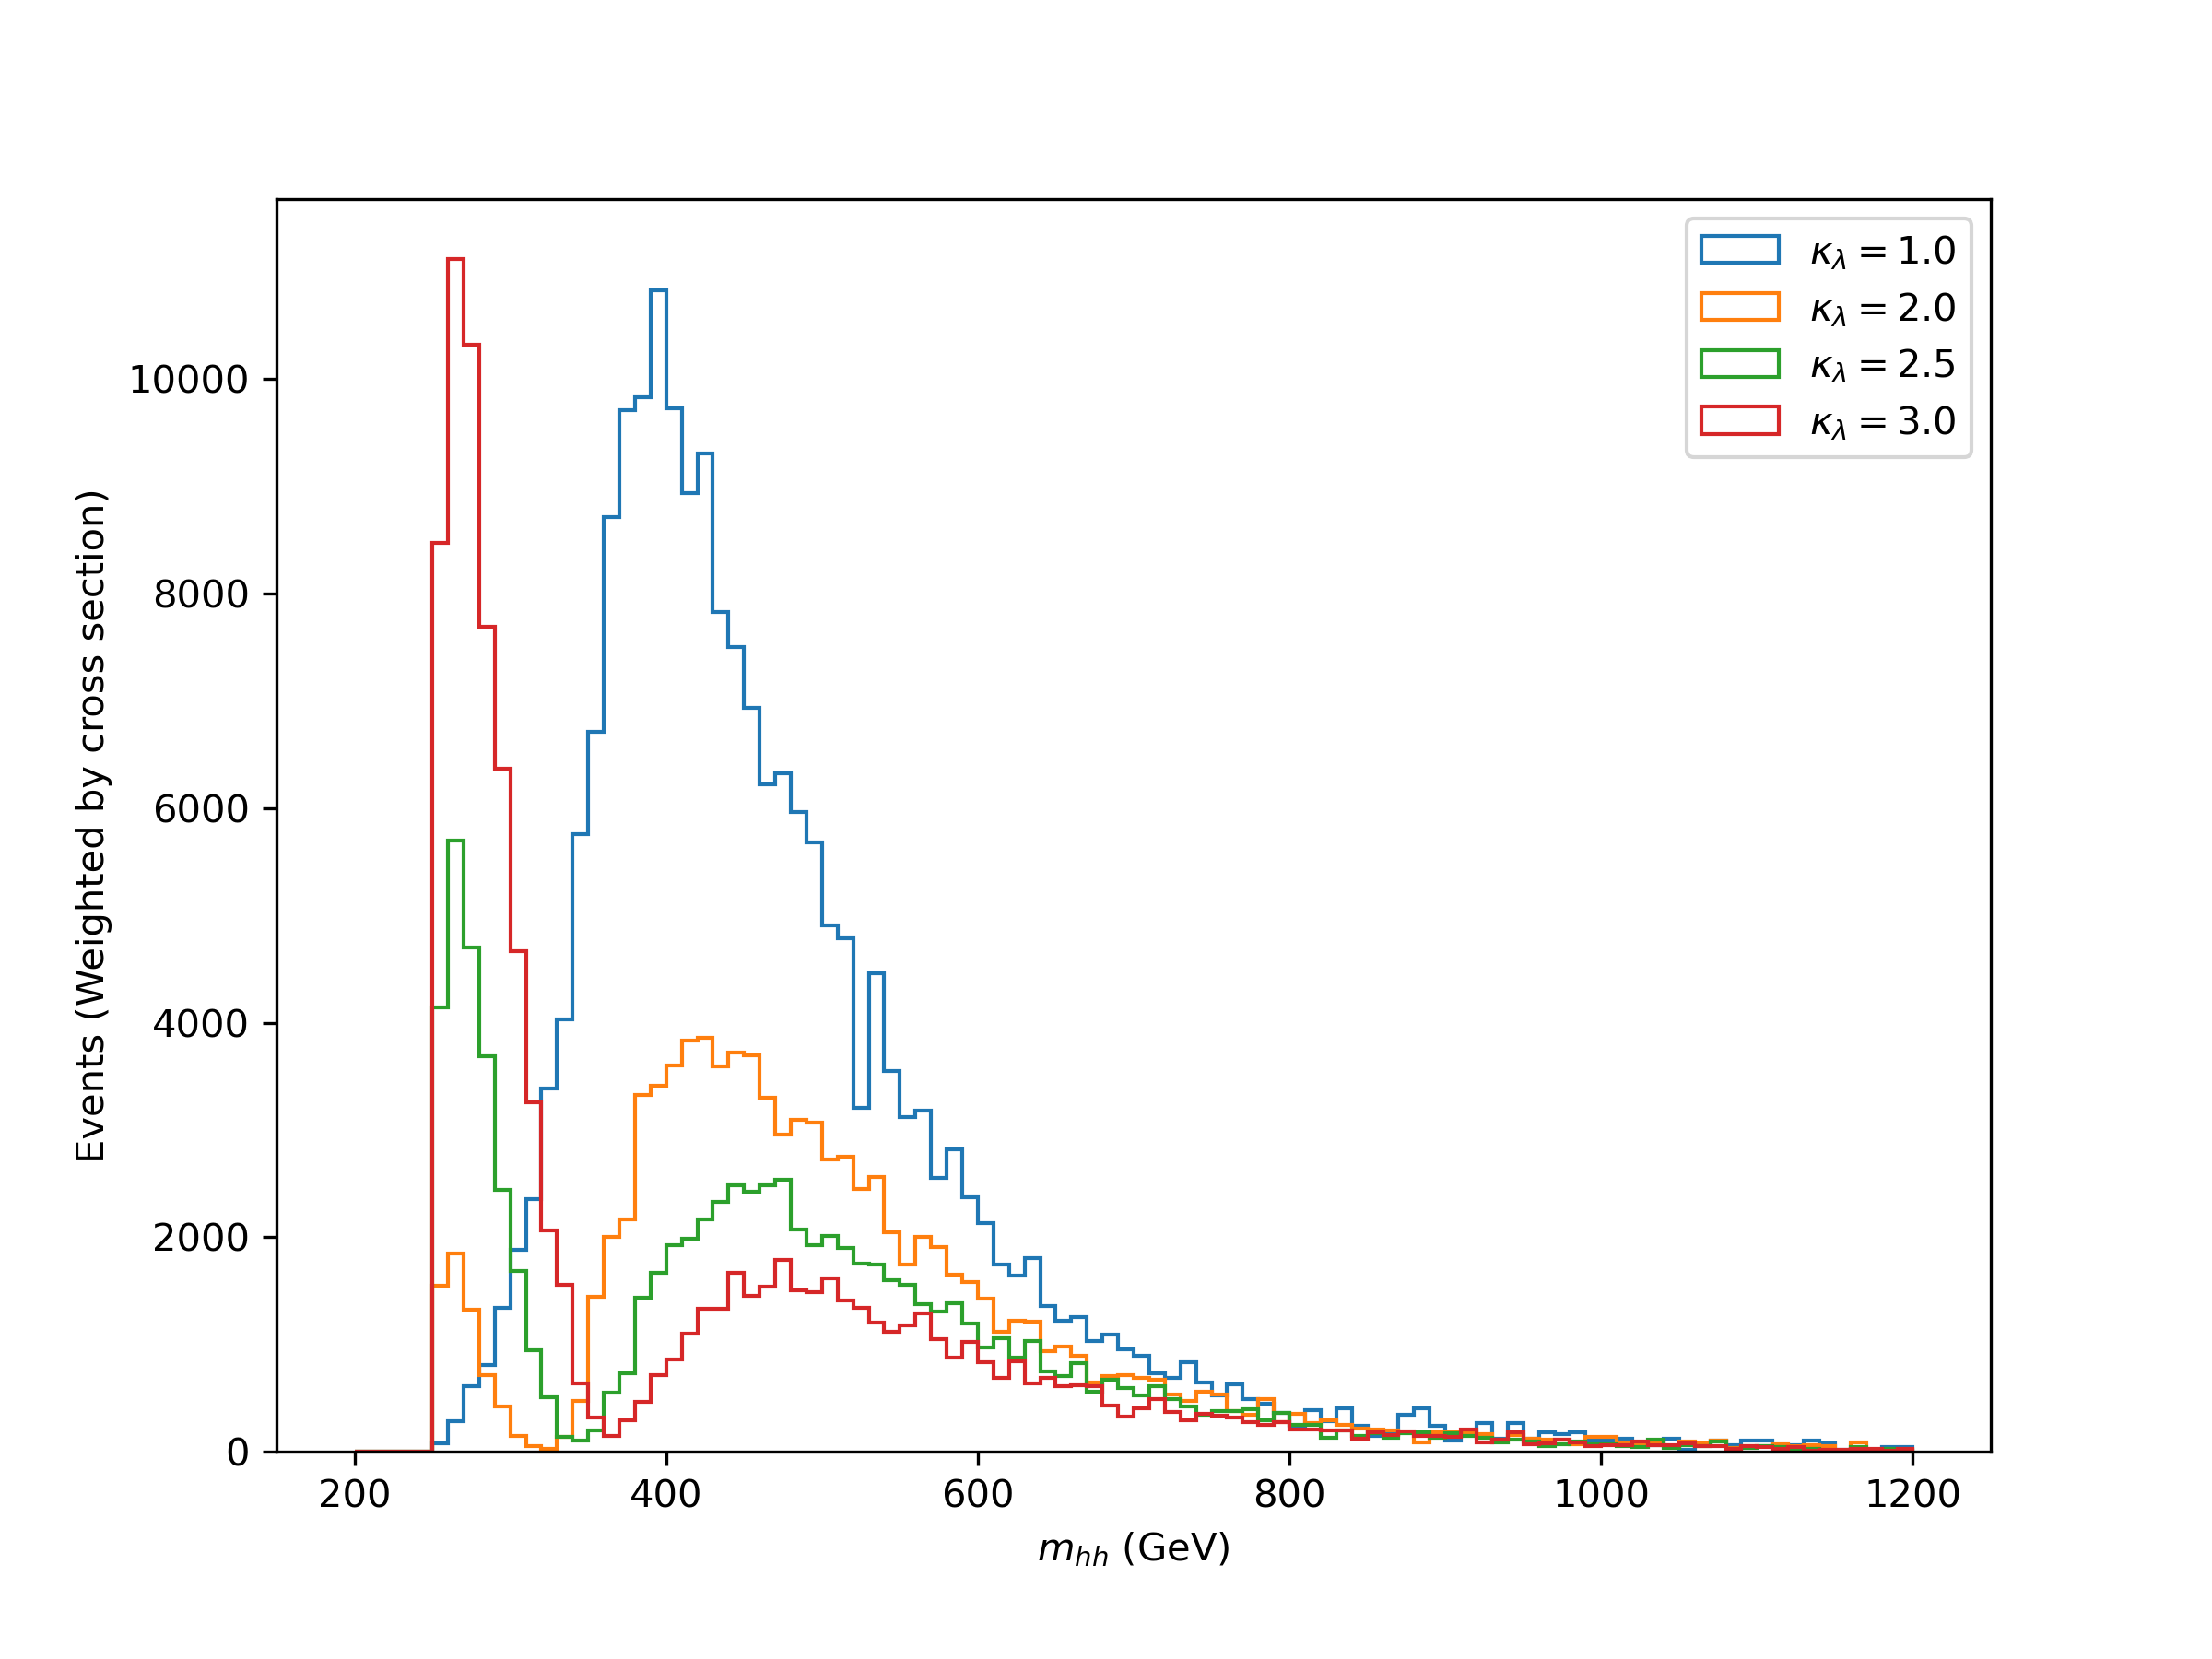
\includegraphics[width=0.49\textwidth]{di-Higgs-SM-kappa-mhh-my-data.png}
			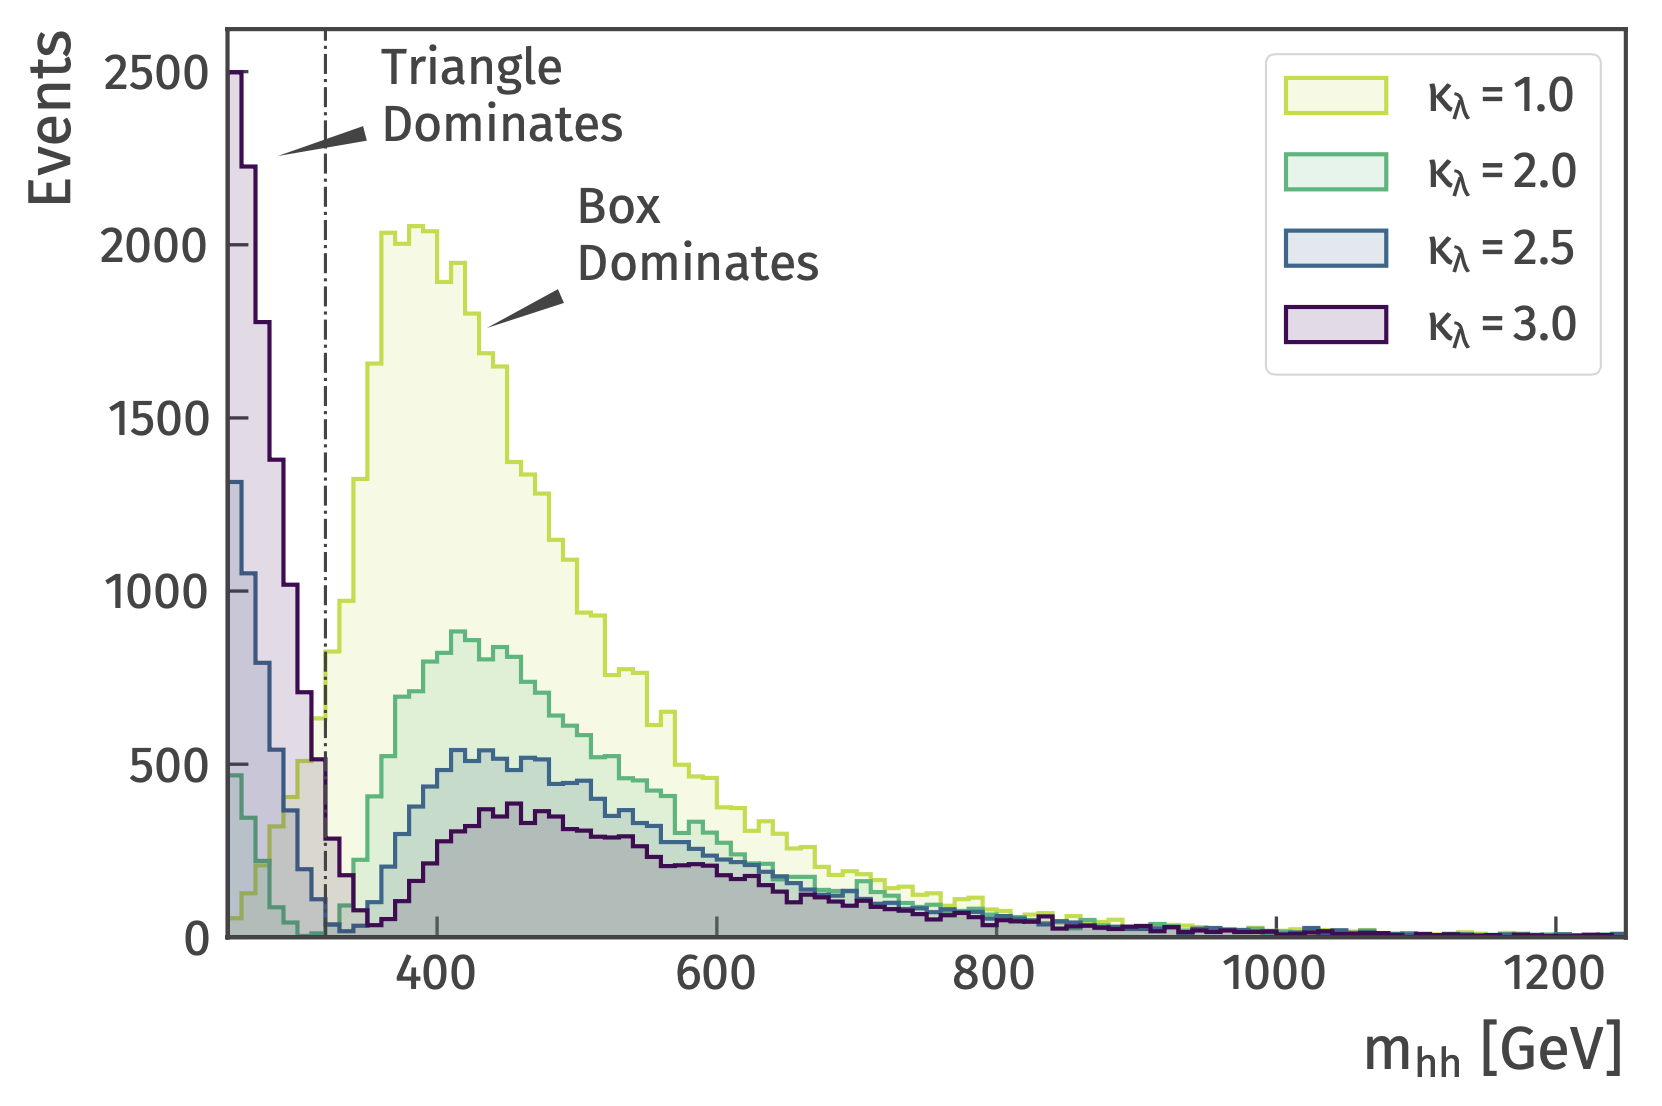
\includegraphics[width=0.49\textwidth]{di-Higgs-SM-kappa-mhh-ref.png}
			\caption{The $m_{hh}$ distribution with various $\kappa_\lambda$. The bin height is weighted by the cross section.}
			\label{fig:di-Higgs-SM-kappa-mhh}
		\end{figure}

		Figure \ref{fig:di-Higgs-SM-kappa-mhh-14TeV} and \ref{fig:di-Higgs-SM-kappa-pth-14TeV} are generated at $\sqrt{s} = 14 \text{ TeV}$. 
		\begin{figure}[htpb]
			\centering
			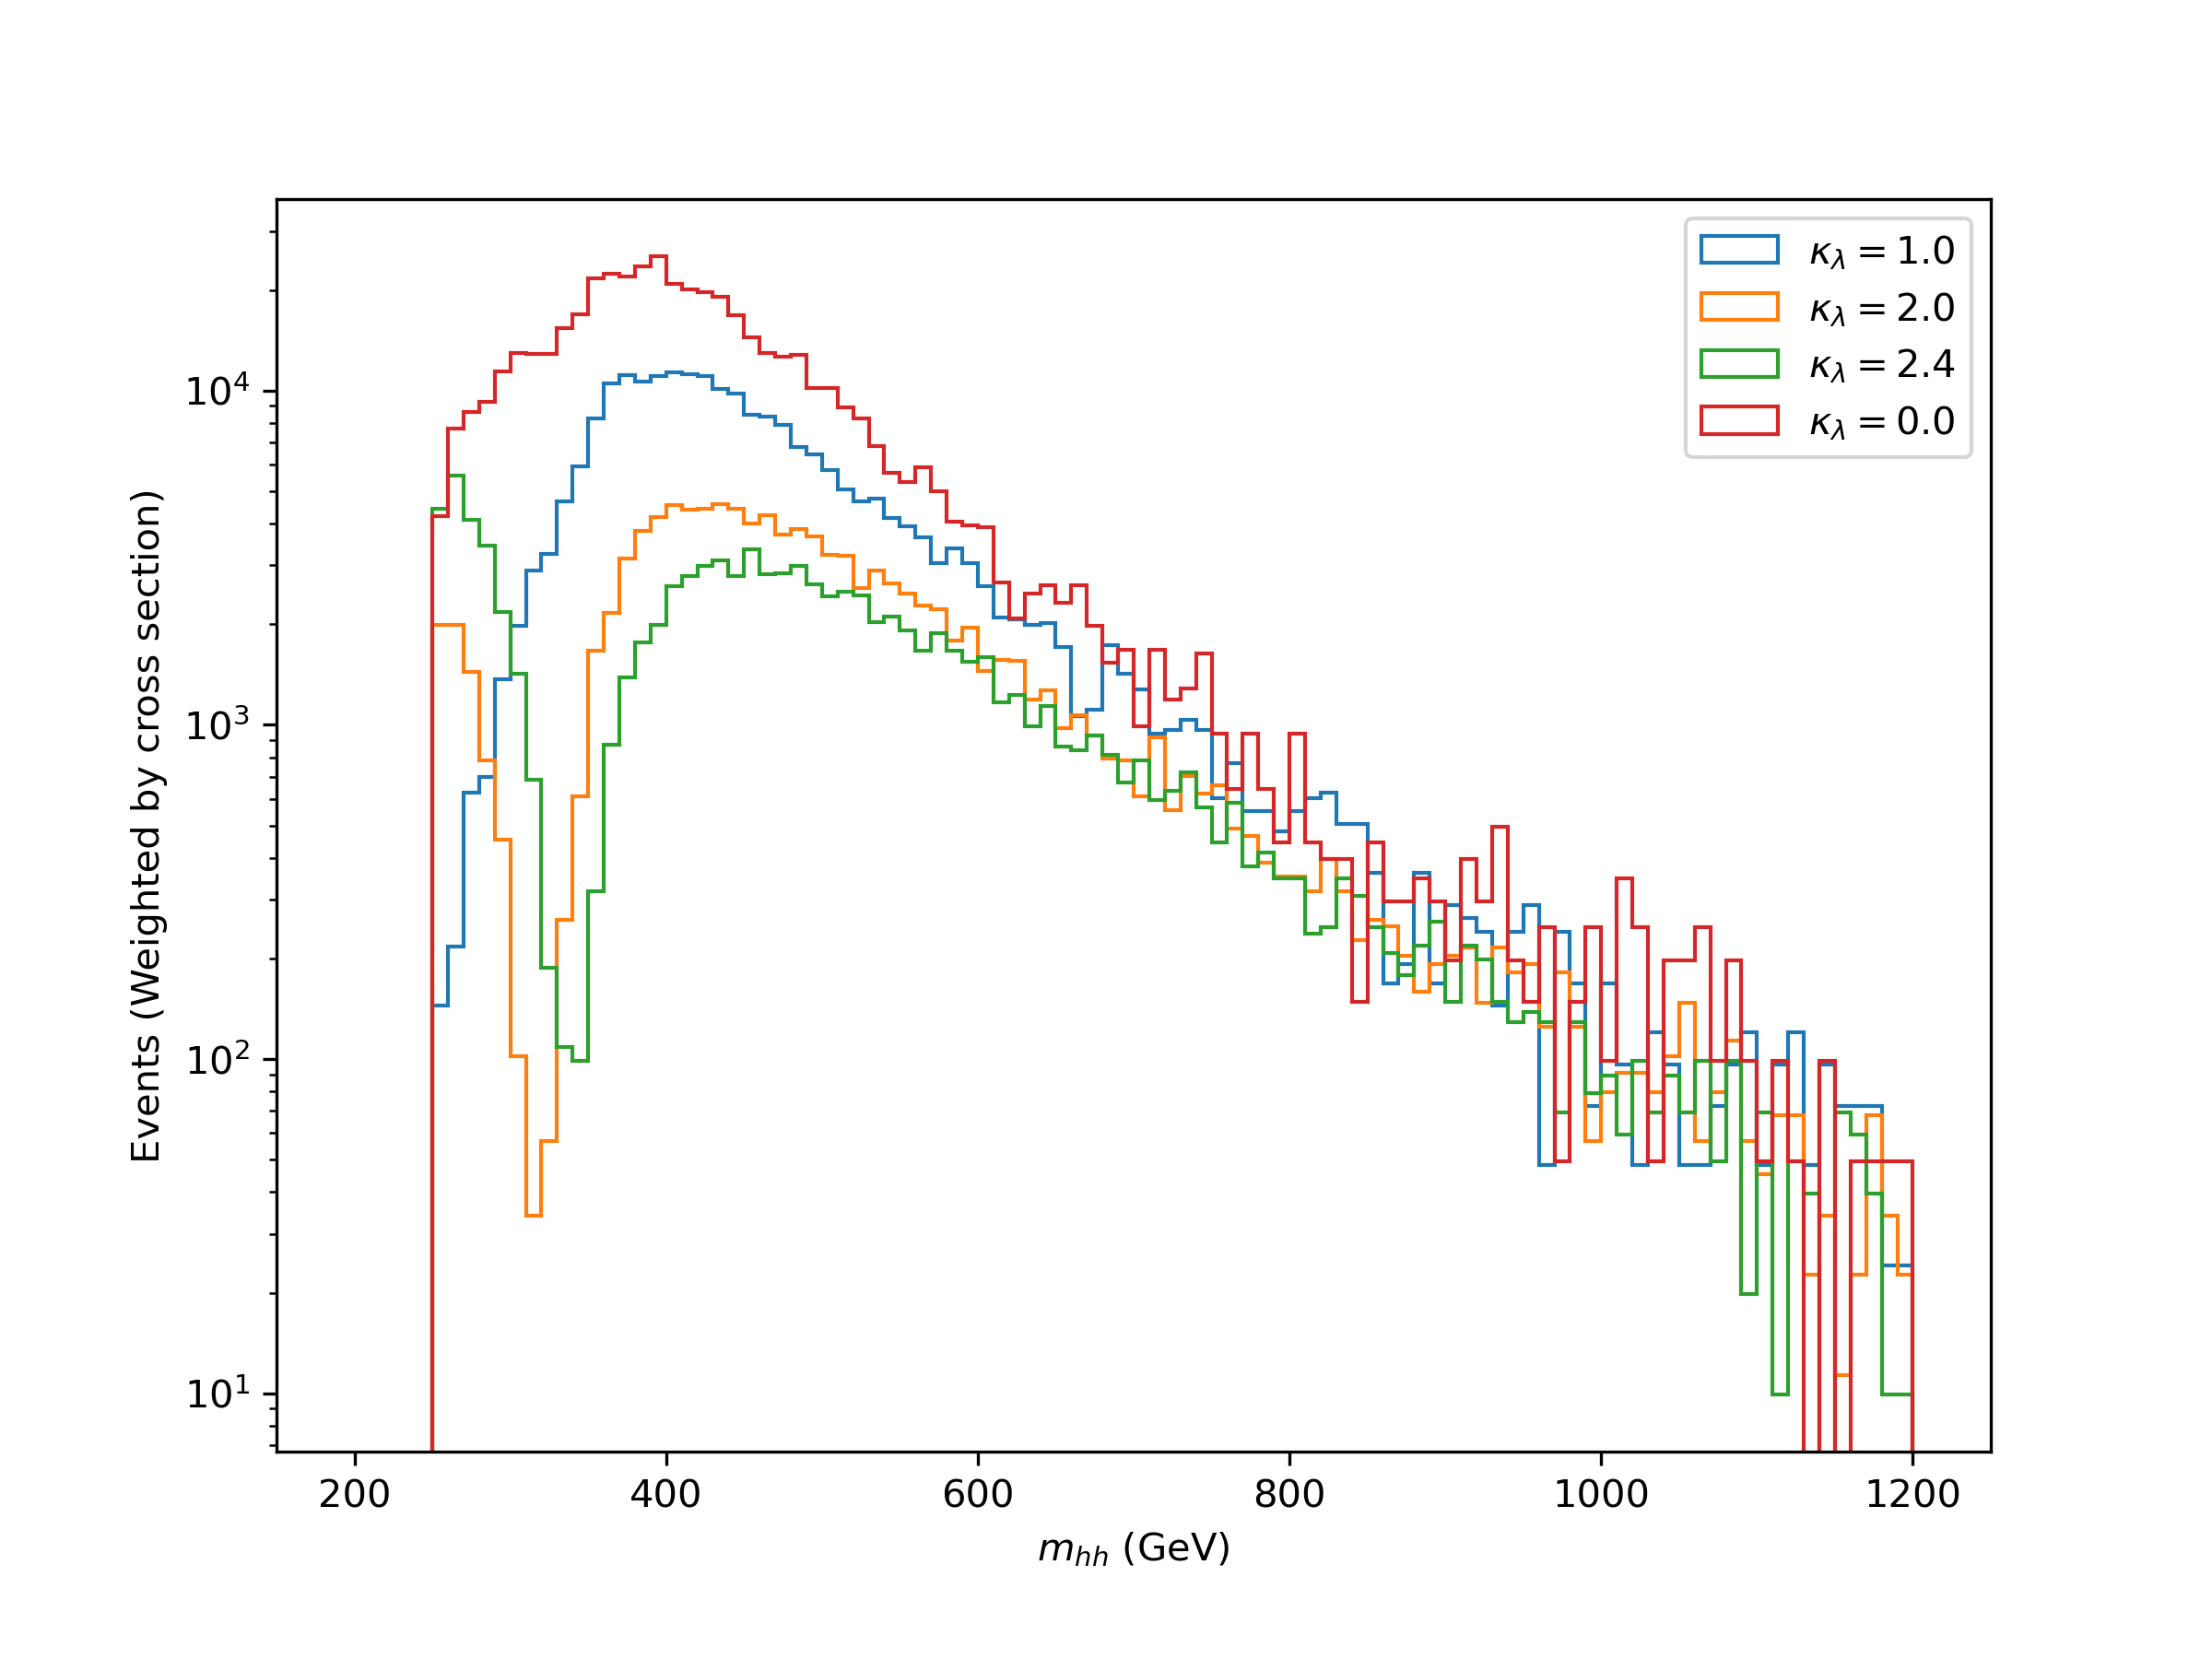
\includegraphics[width=0.49\textwidth]{di-Higgs-SM-kappa-mhh-14TeV-my-data.png}
			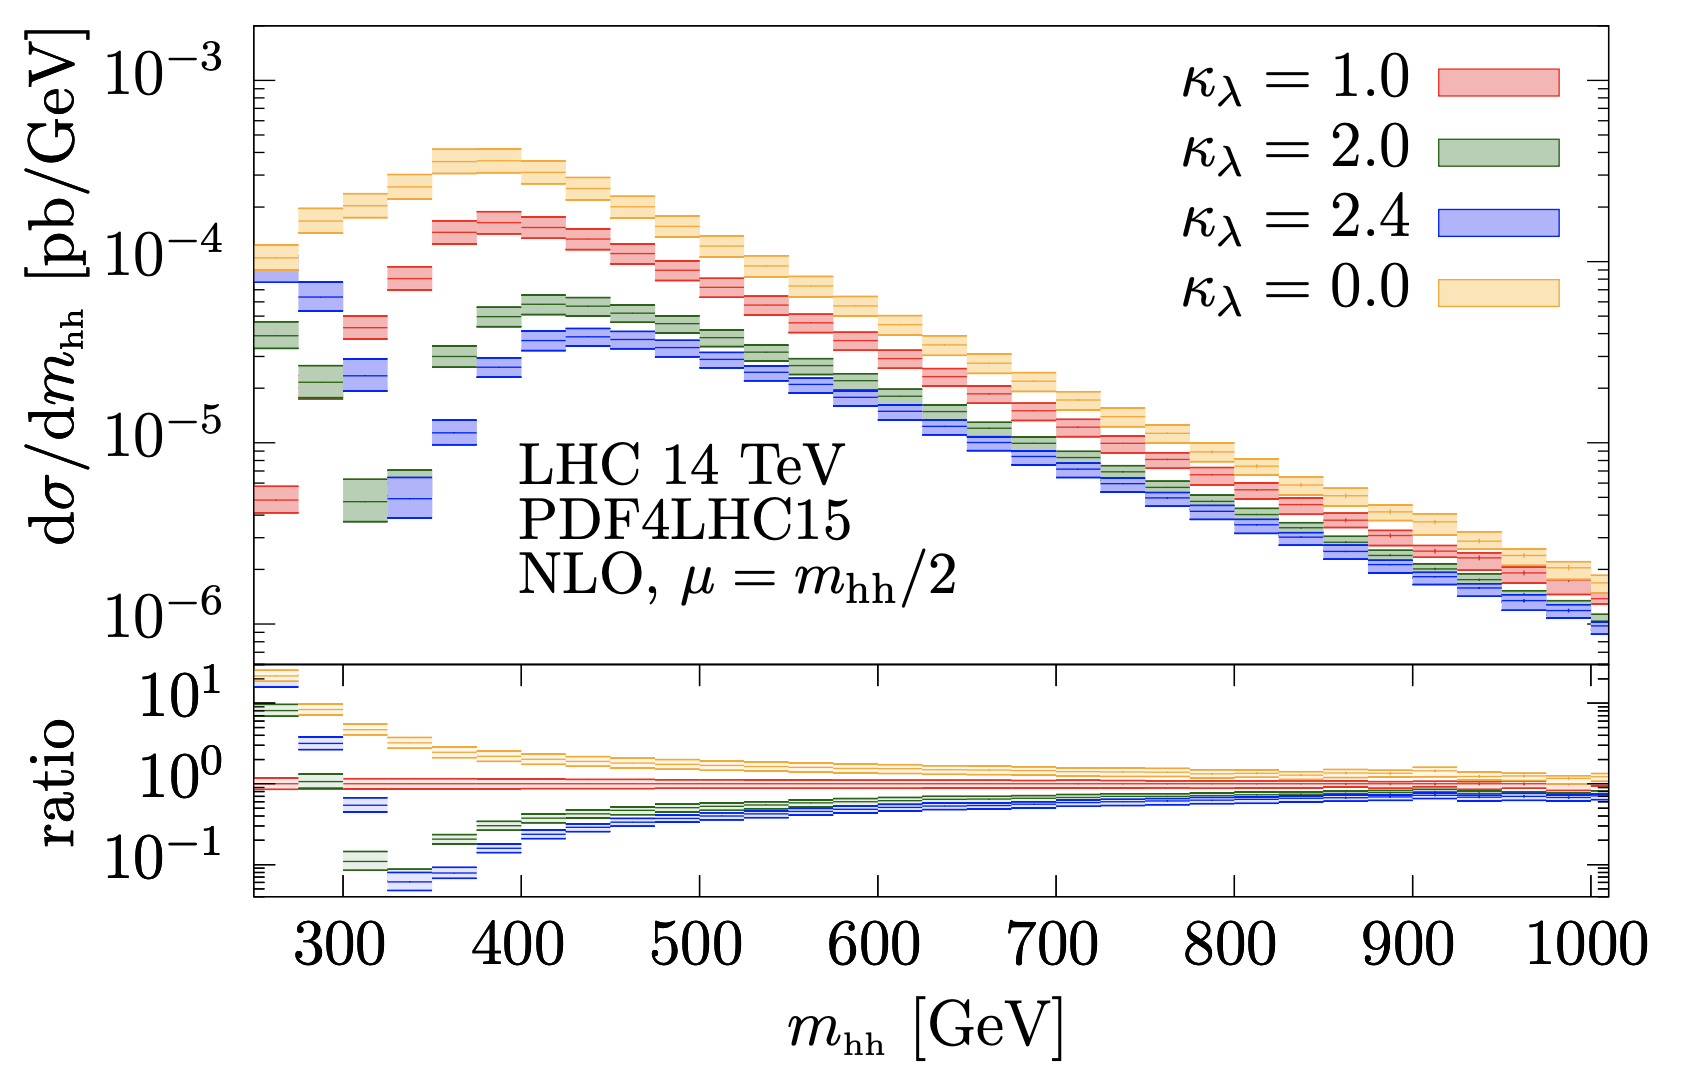
\includegraphics[width=0.49\textwidth]{di-Higgs-SM-kappa-mhh-14TeV-ref.png}
			\caption{The $m_{hh}$ distribution with various $\kappa_\lambda$. The bin height is weighted by the cross section.}
			\label{fig:di-Higgs-SM-kappa-mhh-14TeV}
		\end{figure}
		\begin{figure}[htpb]
			\centering
			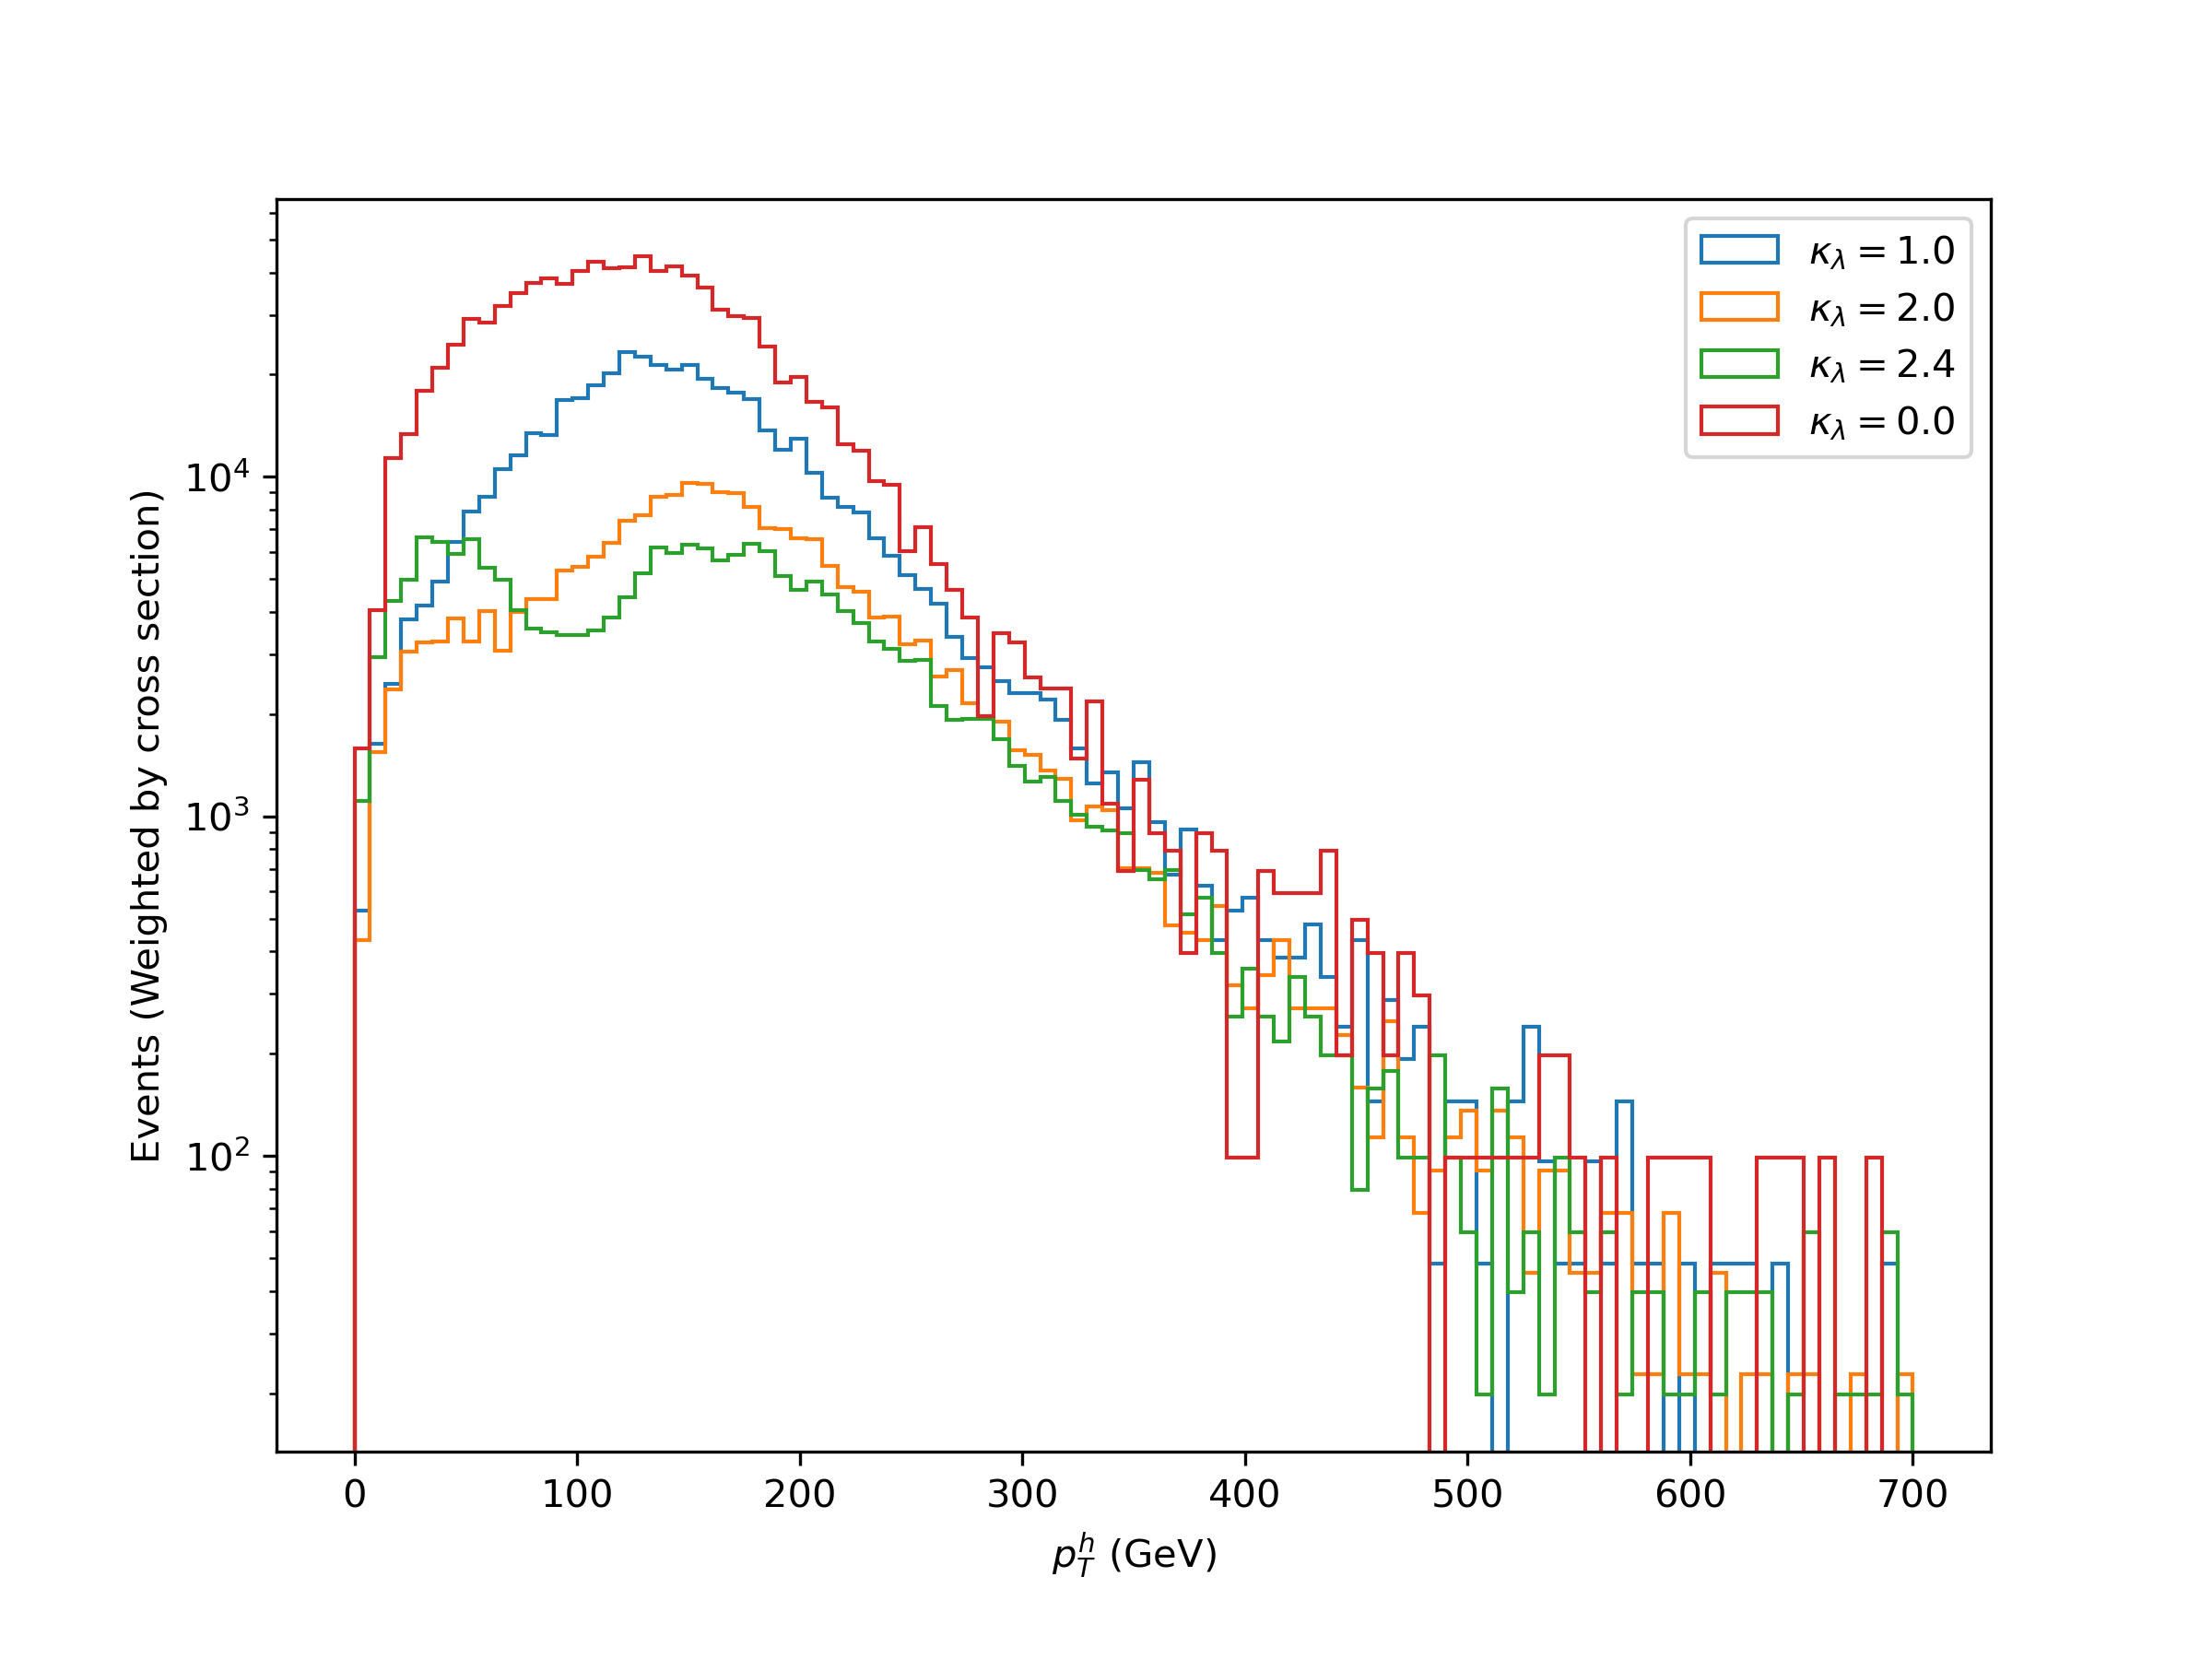
\includegraphics[width=0.49\textwidth]{di-Higgs-SM-kappa-pth-14TeV-my-data.png}
			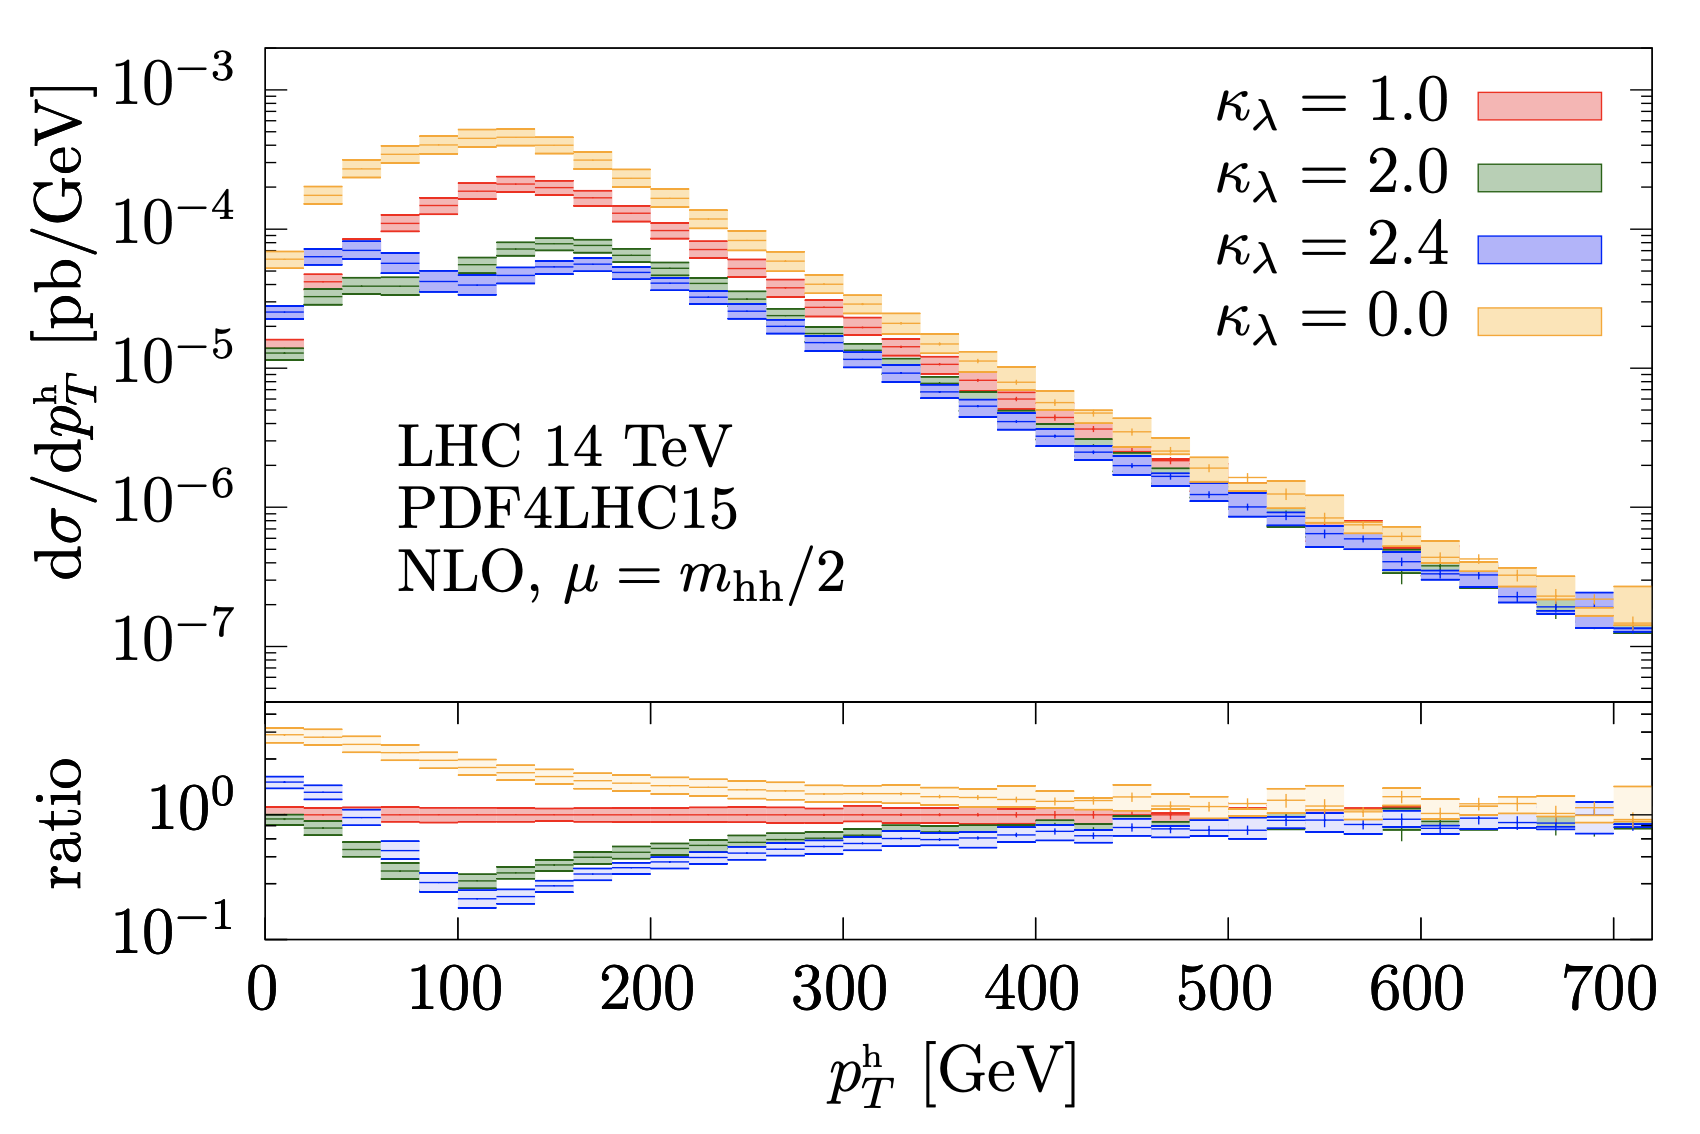
\includegraphics[width=0.49\textwidth]{di-Higgs-SM-kappa-pth-14TeV-ref.png}
			\caption{The $p_\text{T}^{h}$ distribution with various $\kappa_\lambda$. The bin height is weighted by the cross section.}
			\label{fig:di-Higgs-SM-kappa-pth-14TeV}
		\end{figure}

	% subsection di_Higgs_sample_generating_results (end)		
% section generate_di_higgs_samples_in_sm (end)	
\section{Non-resonant di-Higgs event selection}% (fold)
\label{sec:non_resonant_di_higgs_event_selection}
	\subsection{Sample}% (fold)
	\label{sub:sample}
		Non-resonant Higgs pair process is generated by MadGraph. Then pass to Pythia for showering and hadronization. Then pass to Delphes for detector simulation.

		Jets are reconstructed using the anti-$k_t$ algorithm with radius parameter $R = 0.4$.

		The b-tagging part in the Delphes card is changed such that same as the DL1r b-tagger at 77\% WP.  The b-jet efficiency is set to 0.77. The c-jet missing rate is set to 0.204. The light jet missing rate is set to 0.0077.
	% subsection sample (end)

	\subsection{Event selection}% (fold)
	\label{sub:event_selection}
		Reference: \href{https://cds.cern.ch/record/2811390/files/ATLAS-CONF-2022-035.pdf}{ATLAS CONF Note CONF-HDBS-2022-35}

		The selection steps:
		\begin{itemize}
			\item Four tag: The event contains at least 4 b-tagged anti-$k_t$ $R = 0.4$ jets with $p_\text{T} > \text{40 GeV}$ and $\abs{\eta} < 2.5$.
			\item The four jets with the highest $p_\text{T}$ are paired to construct two Higgs boson candidates.
			\item $\text{min-}\Delta R$ pairing method: Choose the pairing in which the higher-$p_\text{T}$ jet pair has the smallest $\Delta R$ separation.
			\item Higgs Eta: 
			\[
				\abs{\Delta\eta_{HH}} < 1.5
			\] 
			\item Top veto: Every possible pair of jets with $p_\text{T} > \text{40 GeV}$ and $\abs{\eta} < 2.5$, including those that were not selected for the $H$ candidates, to form ``$W$ candidates''. ``Top quark candidates'' are built by pairing $W$ candidates with each remaining jet that was selected for $H$ candidates. The quantity $X_{Wt}$ is defined as
			\[
				X_{Wt} = \sqrt{\left( \frac{m_{W} - \text{80.4 GeV}}{0.1 m_{W}} \right)^2 + \left(\frac{m_{t} - \text{172.5 GeV}}{0.1 m_{t}} \right)^2} 
			\] 
			Events with the smallest $X_{Wt} < 1.5$ are vetoed.

			\item Signal region:
			\[
				X_{HH} = \sqrt{\left( \frac{m_{H_1}- \text{124 GeV}}{0.1 m_{H_1}} \right)^2 + \left(\frac{m_{H_2} - \text{117 GeV}}{0.1 m_{H_2}} \right)^2} < 1.6
			\]
			
		\end{itemize}
		\begin{table}[htpb]
			\centering
			\caption{The selection passing rate and efficiency at each stage. The b-tagging part is the same as the DL1r 77\% WP. }
			\label{tab:signal_selection_efficiency__DL1r}
			\begin{tabular}{l|cc|cc}
							  & \multicolumn{2}{|c|}{ATLAS} & \multicolumn{2}{|c}{My sample} \\
				Cut           & pass rate       & efficiency       & pass rate         & efficiency         \\ \hline
				Four tag      & 0.0649 & 0.0649 & 0.0852 & 0.0852 \\
				Higgs Eta     & 0.0543 & 0.8360 & 0.0688 & 0.8074 \\
				Top veto      & 0.0456 & 0.8401 & 0.0553 & 0.8044 \\
				Signal region & 0.0220 & 0.4818 & 0.0181 & 0.3283 \\
			\end{tabular}
		\end{table}

		Correct selection:
		Consider the events in which four jets can be matched one-to-one (within $\Delta R < 0.3$) to the four b-quarks decayed from the Higgs bosons. For the highest $p_\text{T} $ there are 89\% of simulated signal events reaching this selection.	

		Correct pairing: Consider the correct selection events, for $\text{min-}\Delta R$ pairing method there 85\% of events are correctly paired.

		Figure \ref{fig:Higgs_mass_new} shows the Higgs mass distribution. There is a deviation between the mass distribution peak and the signal region's center.  
		\begin{figure}[htpb]
			\centering
			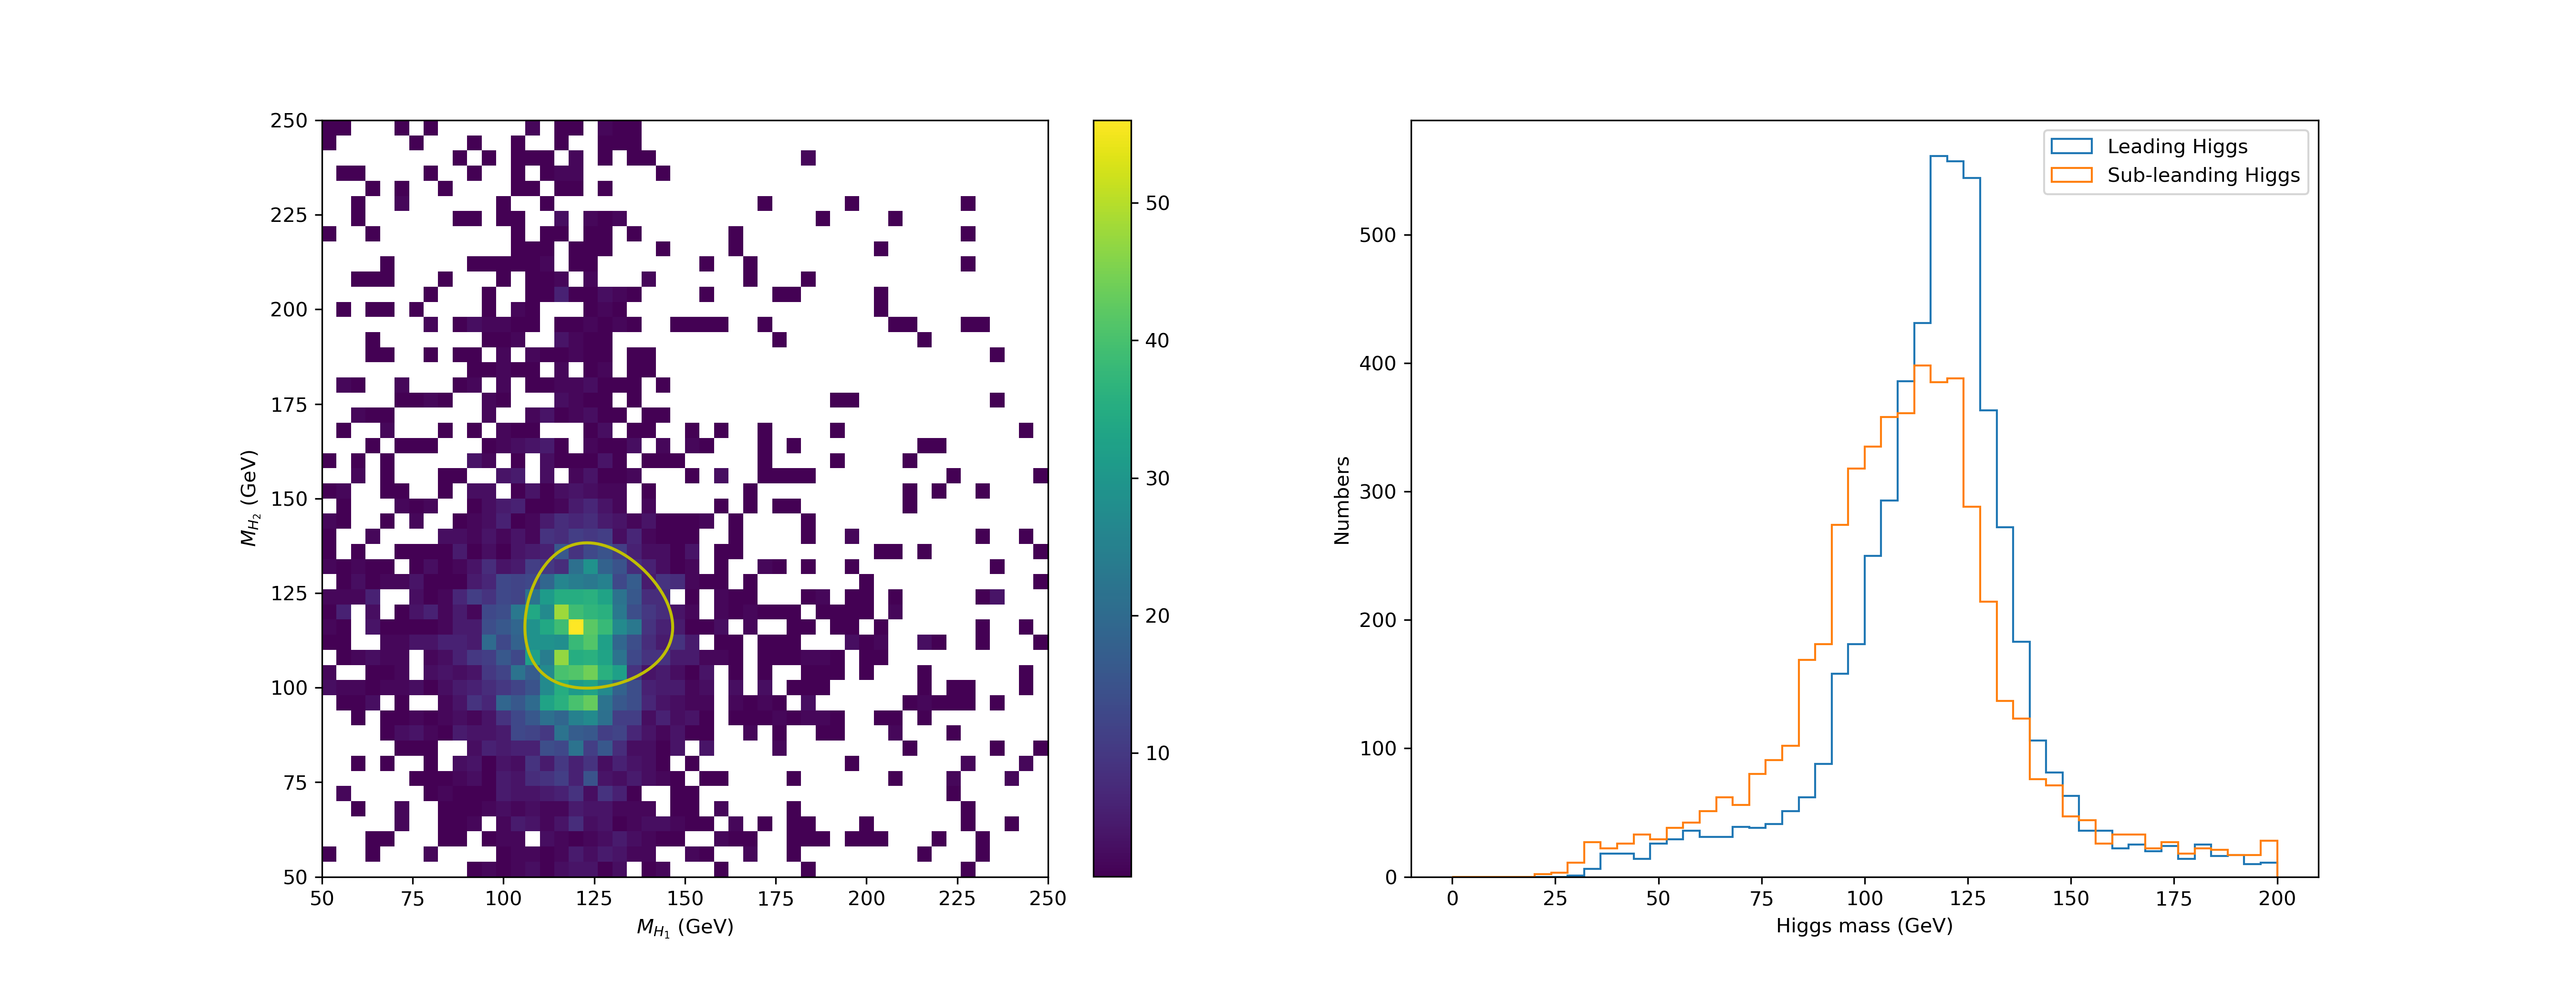
\includegraphics[width=0.95\textwidth]{Higgs_mass_new_s.png}
			\caption{The mass plane and distribution for Higgs candidate.}
			\label{fig:Higgs_mass_new}
		\end{figure}

		\subsubsection{Old method}% (fold)
		\label{subs:subsubsection_name}
			Reference: \href{https://arxiv.org/pdf/1804.06174.pdf}{Search for pair production of Higgs bosons in the $b\overline{b}b\overline{b}$ final state using proton-proton collisions at $\sqrt{s} = \text{13 TeV}$ with the ATLAS detector}

			The selection steps:
			\begin{itemize}
			\item Four tag: The event contains at least 4 b-tagged anti-kt small-$R$ ($R = 0.4$) jets with $p_\text{T} > \text{40 GeV}$ and $\abs{\eta} < 2.5$. The four jets with the highest b-tagging score are paired to construct two Higgs boson candidates.
			\item The four jets with the highest $p_\text{T}$ are paired to construct two Higgs boson candidates in my samples.
			\item Delta R: Pairing jets to Higgs boson candidate need to satisfy the following requirements:
			\[
				\left.
				\begin{array}{c}
					\dfrac{\text{360 GeV}}{m_\text{4j}} - 0.5 < \Delta R_{jj,\text{lead}} < \dfrac{\text{653 GeV}}{m_{\text{4j}}} + 0.475 \\
					\dfrac{\text{235 GeV}}{m_\text{4j}}  < \Delta R_{jj,\text{subl}} < \dfrac{\text{875 GeV}}{m_{\text{4j}}} + 0.35 
				\end{array} 
				\right\} \text{ if } m_{\text{4j}} <  \text{1250 GeV}
			\] 
			\[
				\left.
				\begin{array}{c}
					0 < \Delta R_{jj,\text{lead}} < 1 \\
					0 < \Delta R_{jj,\text{subl}} < 1 
				\end{array} 
				\right\} \text{ if } m_{\text{4j}} >  \text{1250 GeV}
			\] 
			\item If there are more than 2 pairings satisfy the Delta R requirement. Calculate $D_{HH}$
			\[
				D_{HH} = \frac{\abs{m_{\text{2j}}^{\text{lead}} - \frac{120}{110} m_{\text{2j}}^{\text{subl}}}}{\sqrt{1 + \left( \frac{120}{110} \right)^2}}
			\] 
			the pairing with the smallest value of $D_{HH}$ is chosen.
			\item Higgs PT: 
			\begin{align*}
				p_{\text{T}}^{\text{lead}} &> m_{\text{4j}} \times 0.5 - \text{103 GeV} \\
				p_{\text{T}}^{\text{subl}} &> m_{\text{4j}} \times 0.33 - \text{73 GeV} \\
			\end{align*}
			\item Higgs Eta: 
			\[
				\abs{\Delta\eta_{HH}} < 1.5
			\] 
			\item Signal region:
			\[
				X_{HH} = \sqrt{\left( \frac{m_{\text{2j}}^{\text{lead}} - \text{120 GeV}}{0.1 m_{\text{2j}}^{\text{lead}}} \right)^2 + \left(\frac{m_{\text{2j}}^{\text{subl}} - \text{110 GeV}}{0.1 m_{\text{2j}}^{\text{subl}}} \right)^2} < 1.6
			\]
			\item Top veto: Every possible pair of jets with $p_\text{T} > \text{40 GeV}$ and $\abs{\eta} < 2.5$, including those that were not selected for the $H$ candidates, to form ``$W$ candidates''. ``Top quark candidates'' are built by pairing $W$ candidates with each remaining jet that was selected for $H$ candidates
			\[
				X_{Wt} = \sqrt{\left( \frac{m_{W} - \text{80 GeV}}{0.1 m_{W}} \right)^2 + \left(\frac{m_{t} - \text{173 GeV}}{0.1 m_{t}} \right)^2} 
			\] 
			Events with the smallest $X_{Wt} < 1.5$ are vetoed.

			\end{itemize}

			The results are in Table \ref{tab:signal_selection_efficiency_MV2c10}.
			\begin{table}[htpb]
				\centering
				\caption{The selection passing rate and efficiency at each stage.}
				\label{tab:signal_selection_efficiency_MV2c10}

				\begin{tabular}{l|cc|cc}
								  & \multicolumn{2}{|c|}{ATLAS} & \multicolumn{2}{|c}{My sample} \\
					Cut           & pass rate       & efficiency       & pass rate         & efficiency         \\ \hline
					Four tag      & 0.0490 & 0.0490 & 0.0563 & 0.0563 \\
					Delta R       & 0.0448 & 0.9143 & 0.0471 & 0.8370 \\
					Higgs PT      & 0.0422 & 0.9420 & 0.0446 & 0.9480 \\
					Higgs Eta     & 0.0380 & 0.9005 & 0.0398 & 0.8911 \\
					Signal region & 0.0193 & 0.5079 & 0.0170 & 0.4280 \\
					Top veto      & 0.0179 & 0.9275 & 0.0145 & 0.8537
				\end{tabular}
			\end{table}

		% subsubsection subsubsection_name (end)	

	% subsection event_selection (end)	
	
% section non_resonant_di_higgs_event_selection (end)		
\end{document} 
